\chapter{Fondamentali}
L'identificazione della posizione all'interno di un edificio si svolge in 3 fasi:
\begin{enumerate}
	\item Scansione dell'ambiente
	\item Costruzione di un modello
	\item Ricerca della posizione
\end{enumerate}

Nelle successive 3 sezioni discuteremo dei fondamenti teorici dietro ciascuna di queste fasi.

\section{Fase 1: Raccoglimento ed elaborazione dei dati}
Il raccoglimento dei dati avviene tramite il magnetometro del nostro \textit{smartphone} da cui viene catturato diverse volte in un secondo il campo magnetico intorno ad esso.
Ad ogni onda magnetica viene assegnata una \textit{label}: un numero che identifica univocamente una parte dell'ambiente chiuso il cui uso verra' definito durante la fase di costruzione del modello.

\subsection{Onde Magnetiche}
Le onde magnetiche sono un vettore di 3 elementi, quindi in $R^3$ che classifica. Il primo valore rappresenta la forza del campo magnetico lungo l'asse X, il secondo lungo Y ed il terzo lungo Z.


\begin{figure}[H]
	\centering
	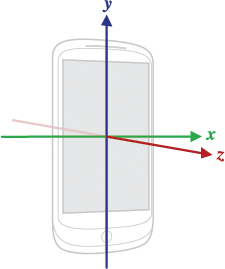
\includegraphics[width=0.20\linewidth]{./img/axis_magnetic_field.png}
	\caption{Assi x, y, z centrati sul cellulare}
	\label{fig:axis_magnetic_field}
\end{figure}
I tre valori sono espressi in $ \mu T $ (micro Tesla), unita' di misura della densita' di un flusso magnetico.
Le onde magnetiche raccolte sono dati continui sia positivi che negativi. L'intensita' dell'onda deriva dalla distorsione del campo magnetico generata dagli oggetti statici intorno al punto e dipende anche dalla velocita' con cui ci muoviamo per cui, per semplicita', assumeremo d'ora in poi una velocita' costante di 3 piedi al secondo.

\begin{figure}[H]
	\centering
	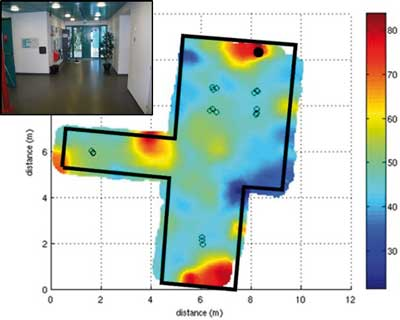
\includegraphics[width=0.7\linewidth]{img/magnetic_field_map}
	\caption[Un esempio di mappa del campo magnetico]{Mappa del campo magnetico all'universita' di Oulu: Discus Entrance hall}
	\label{fig:magneticfieldmap}
\end{figure}

\subsection{Estrazione del magnitudo}
Per estrarre l'intensit\`{a} di ogni onda magnetica eseguiamo semplicemente la norma euclidea di un vettore:\\
\begin{center}
	$ \sqrt{x^2 + y^2 + z^2}$
\end{center}

\subsection{Raggruppamento}
Le onde magnetiche con la stessa \textit{label} vengono raggruppate in \textit{fingerprints}, insiemi di dimensione prefissata. A livello logico, ogni \textit{fingerprint} cerca di identificare univocamente un punto all'interno di una zona, identificata con una \textit{label}. L'insieme di \textit{fingerprints} quindi, cerca di distinguere, tramite le caratteristiche dei campi elettromagnetici di ciascun punto, ogni \textit{label} dall'altra.

\subsection{Estrazione degli attributi}
Per ogni \textit{fingerprint}, l'estrazione degli attributi consiste nel creare nuovi attributi in funzione di quelli gia' esistenti. Una possibile applicazione e' l'estrazione di variabili statistiche dagli attributi gia' presenti come per esempio:
\begin{itemize}
	\item Media
	\item Varianza
	\item Deviazione standard
	\item Mediana
	\item Media troncata
	\item Coefficiente di variazione
	\item Massimo
	\item Minimo
	\item $ 1^{\circ}, 5^{\circ}, 95^{\circ}, 99^{\circ} $ percentile
	\item $ 1^{\circ}, 2^{\circ}, 3^{\circ} $ quartile
\end{itemize}

\subsection{Normalizzazione e standardizzazione}
2 tecniche molto usate per poter confrontare i valori dei nostri attributi in una scala comune sono la normalizzazione e la standardizzazione. La prima centra porta la media dei valori di quell'attributo a 0 e la deviazione standard ad 1 mentre la seconda porta tutti i valori in un intervallo $[0 , 1]$\\
L'equazione della normalizzazione per il j$-$esimo attributo di tipo $x_i$ e' la seguente:
\begin{center}
	$x_{ij} = \dfrac{x_{ij} - \mu_i}{\sigma_i}$
\end{center}
dove $\mu_i$ e' la media per gli attributi di tipo $i$ e $\sigma_i$ la deviazione standard.
Adesso vediamo la standardizzazione:
\begin{center}
	$x_{ij} = \dfrac{x_{ij} - x_{min}}{x_{max} - x_{min}}$
\end{center}

\section{Fase 2: costruzione di un modello}

Dopo aver raccolto ed elaborato le onde magnetiche, un algoritmo creera' un classificatore in grado di assegnare un'etichetta ai nuovi input ricevuti durante l'uso dell'utente finale.
Sono stati utilizzati vari classificatori per cercare il piu' preciso fra tutti. Qui di seguito introdurremo la teoria dietro ad ogni classificatore utilizzato.

\subsection{IA ed Apprendimento}
La definizione secondo wikipedia \footnote{\url{https://it.wikipedia.org/wiki/Intelligenza_artificiale}} di IA e' la seguente:\\
Definizioni specifiche possono essere date focalizzandosi o sui processi interni di ragionamento o sul comportamento esterno del sistema intelligente ed utilizzando come misura di efficacia o la somiglianza con il comportamento umano o con un comportamento ideale, detto razionale:
\begin{itemize}
	\item Agire umanamente: il risultato dell'operazione compiuta dal sistema intelligente non e' distinguibile da quella svolta da un umano.
	\item Pensare umanamente: il processo che porta il sistema intelligente a risolvere un problema ricalca quello umano. Questo approccio � associato alle scienze cognitive.
	\item Pensare razionalmente: il processo che porta il sistema intelligente a risolvere un problema � un procedimento formale che si rif� alla logica.
	\item Agire razionalmente: il processo che porta il sistema
\end{itemize} 
L'apprendimento automatico e' una branca dell'intelligenza artificiale che permette al computer di apprendere da insiemi di dati per generare conoscenza con lo scopo di effettuare previsioni.

\subsection{Tipi di apprendimento}
Esistono 3 tipi di apprendimento:
\begin{itemize}
	\item Apprendimento supervisionato: al calcolatore vengono forniti esempi del tipo (\textbf{x}, y) per poter apprendere. L'obbiettivo della predizione per nuovi input sara' quello di calcolare la variabile dipendente. Y puo' essere sia dicreta che continua: nel primo caso si parla di classificazione, nel secondo di regressione.
	
	
	\begin{figure}[H]
		\centering
		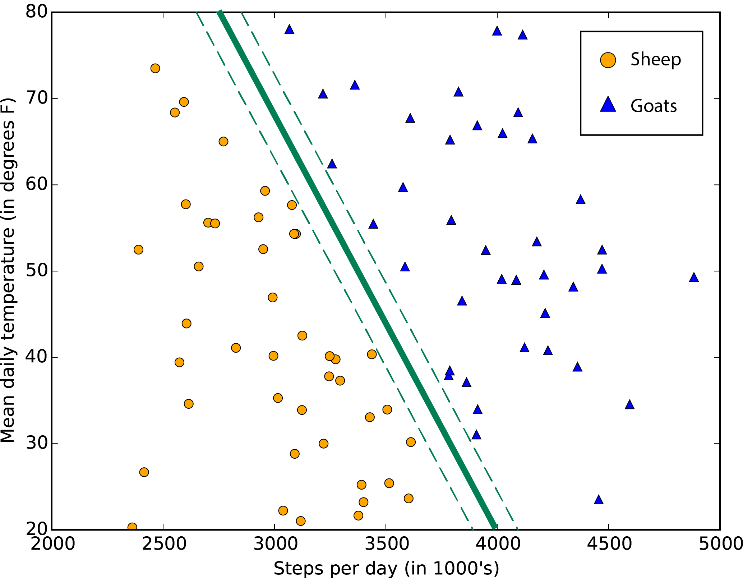
\includegraphics[width=0.7\linewidth]{img/supervised_learning_example}
		\caption{Un esempio grafico di insieme d'addestramento ed una sua classificazione}
		\label{fig:supervisedlearningexample}
	\end{figure}
	
	
	\begin{figure}[H]
		\centering
		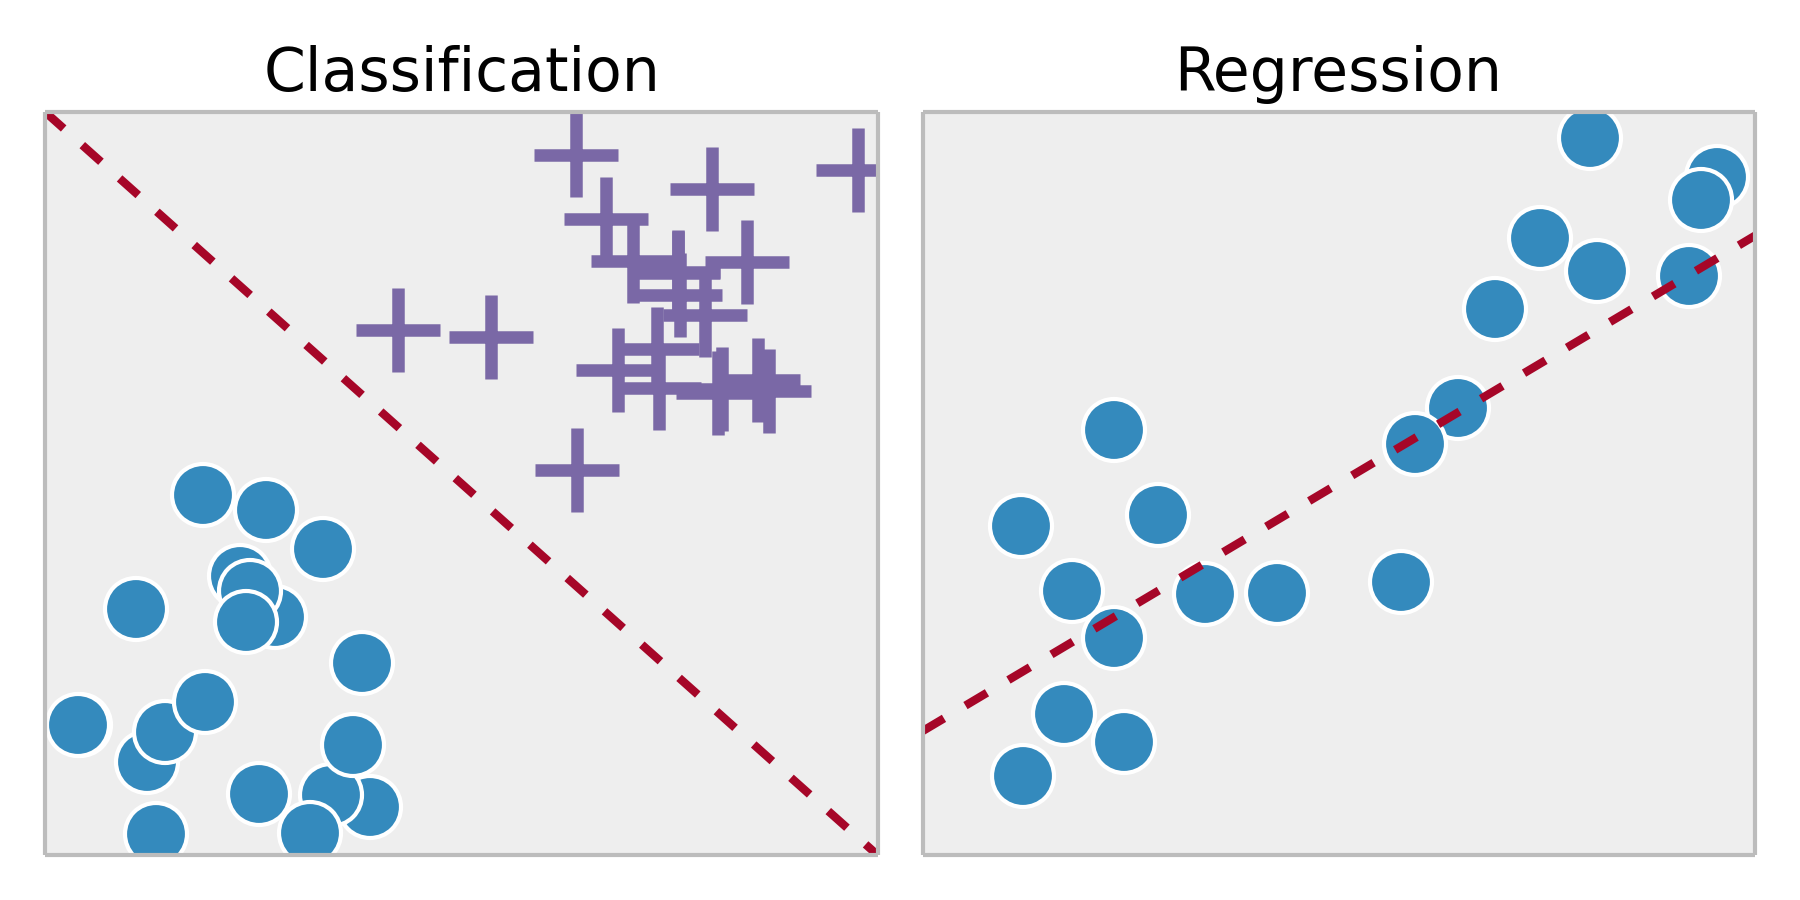
\includegraphics[width=0.7\linewidth]{img/Classification_Regression}
		\caption{Classificazione e regressione a confronto}
		\label{fig:classificationregression}
	\end{figure}

	\item Apprendimento non supervisionato: Gli esempi non contengono una variabile dipendente ma solo un insieme di attributi \textbf{x}. L'obbietto e' quello di inferire pattern nascosti dai dati non etichettati. Un'importante applicazione e' il \textit{clustering}: raggruppare i dati in base ad una similarita' fra di essi.
	
	\begin{figure}[H]
		\centering
		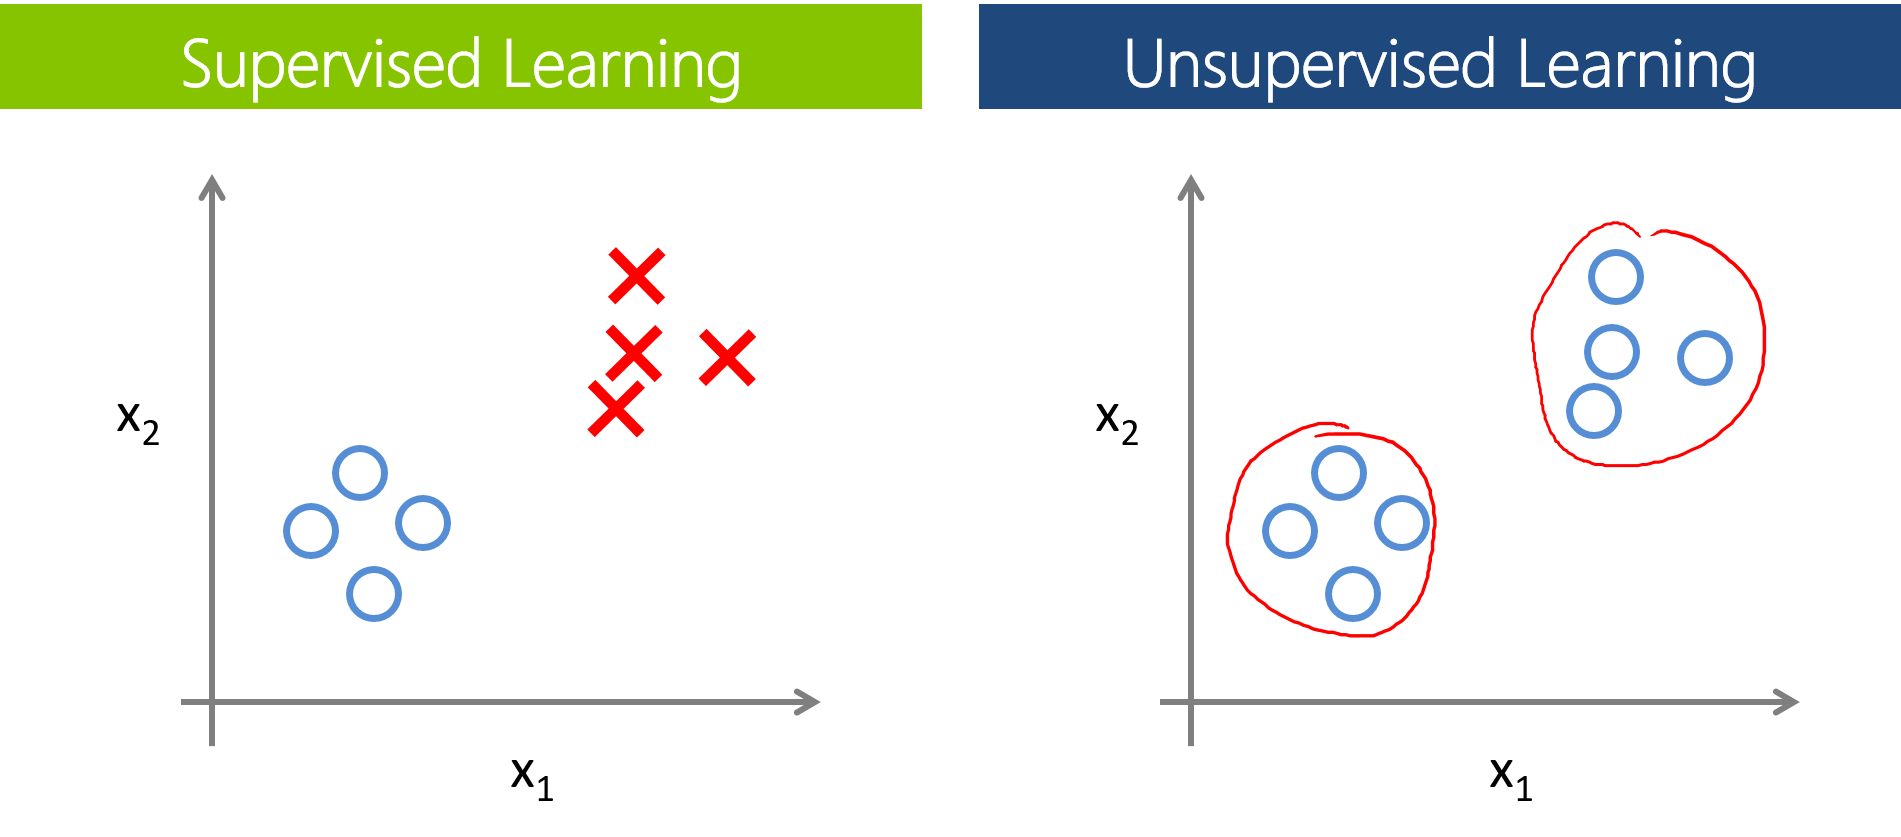
\includegraphics[width=0.7\linewidth]{img/supervised_and_unsupervised_learning}
		\caption{Apprendimento supervisiono e non supervisionato a confronto}
		\label{fig:supervisedandunsupervisedlearning}
	\end{figure}
	
	
	\item Apprendimento con rinforzo: per apprendere viene fornita una funzione ricompensa cioe' una funzione che, data un'azione effettuata dall'agente, restituira' una ricompensa di tipo numerico.
	
	\begin{figure}[H]
		\centering
		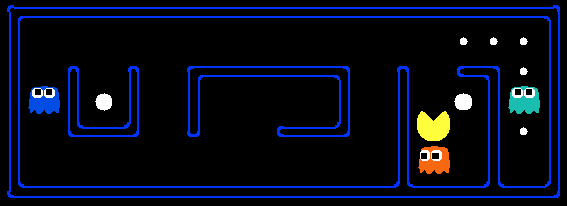
\includegraphics[width=0.7\linewidth]{img/pacman}
		\caption{L'apprendimento con rinforzo e' molto adatto ai giochi, come per esempio pacman}
		\label{fig:pacman}
	\end{figure}
	
	
\end{itemize}


\subsection{Alcune nozioni sull'apprendimento automatico}
\subsubsection{Verifica delle prestazioni}
Per verificare la correttezza del classificatore viene diviso in 2 parti il \textit{dataset} a nostra disposizione: il primo si chiama insieme di addestramento mentre il secondo insieme di test. Il nostro classificatore si allenera' sull'insieme di addestramento, cioe' imparera' dagli esempi come classificare i nuovi input e verifichera' l'efficacia dell'apprendimento sugli esempi in base ad una metrica. Ne esistono diverse ma noi useremo l'accuratezza, ovvero il numero di classificazioni corrette diviso il numero di esempi nell'insieme di test

\begin{figure}[H]
	\centering
	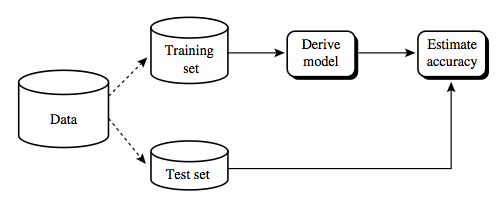
\includegraphics[width=0.7\linewidth]{img/training_test_flow}
	\caption{Un diagramma di flusso che mostra le operazioni di verifica delle prestazioni}
	\label{fig:trainingtestflow}
\end{figure}

\subsubsection{Parametri ed iperparametri}
Ogni modello e' composto da 2 tipi di valori che ne stabiliscono l'efficacia: i parametri, i quali sono determinati internamente dal modello in base al dataset mentre gli iperparametri sono stabiliti dall'utente prima dell'addestramento del modello e  modificano profondamente l'efficacia di predizione. Un esempio che vedremo e' l'iperparametro $k$ del $knn$.




\begin{figure}[H]
	\centering
	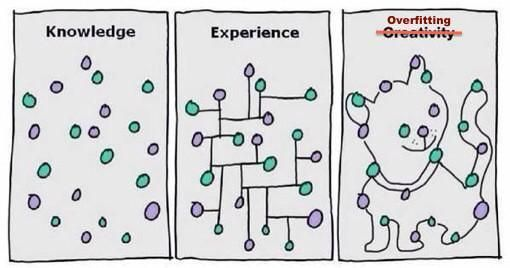
\includegraphics[width=0.7\linewidth]{img/overfitting}
	\caption{Effetti del sovradattamento}
	\label{fig:overfitting}
\end{figure}

\subsubsection{Insieme di validazione}
Per poter stimare il miglior valore da assegnare ai iperparametri del nostro modello, e' opportuno creare un altro insieme dal nostro dataset di partenza: l'insieme di validazione. Notiamo che non e' possibile utilizzare l'insieme di test per questo scopo perche' incapperemo in sovradattamento.

\subsubsection{Cross validation}
Un'alternativa all'insieme di validazione, specie se abbiamo un dataset piccolo, potrebbe essere la \textit{cross validation}. Inizialmente si suddivide l'intero dataset in $n$ parti (di solito 10). A turno una singola parte svolgera' il ruolo di insieme di validazione mentre tutto il resto sara' l'insieme di addestramento. Per valutare le prestazioni verra' fatta una media dell'accuratezza nelle predizioni in modo da avere un risultato piu' preciso rispetto al singolo insieme di validazione. Questa tecnica e' anche utile per evitare sovradattamento sui dati.

\begin{figure}[H]
	\centering
	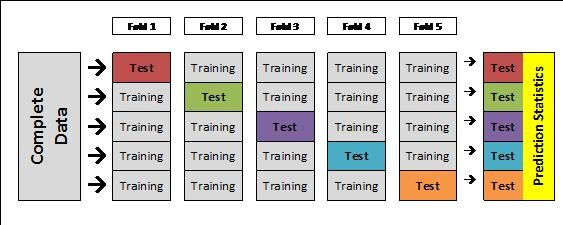
\includegraphics[width=0.7\linewidth]{img/crossvalidation}
	\caption{Rappresentazione grafica della Cross Validation}
	\label{fig:crossvalidation}
\end{figure}

\subsubsection{Rumore e sovradattamento}
Un problema molto comune durante l'addestramento dei classificatori e' il rumore: durante la discriminazione degli esempi, ci potrebbe capitare di avere vari esempi con attributi identici ma con etichetta differente. Una probabile causa potrebbe essere la presenza di errori nei dati mentre una possibile soluzione e' il voto di maggioranza fra gli esempi rimanenti.\\
Un'altro problema e' il sovradattamento: la costruzione di un classificatore consistente con tutti gli esempi porta ad inaccuratezza nei casi reali d'uso. Una possibile causa e' l'utilizzo di attributi irrilevanti nella classificazione. Supponiamo di voler predire l'esito del lancio di un dado e fra gli attributi di avere ora, giorno, mese ed anno; ecco un esempio lampante di sovradattemento. Nei casi reali tuttavia non sono cosi' evidenti gli attributi insignificanti e, per esempio, una tecnica utilizzata  negli alberi di decisione e' la potatura.

\subsection{K Nearest Neightbour}
Uno degli algoritmi piu' semplici di apprendimento automatico, e' il \textit{k-nearest-neightbours} Il KNN viene definito un algoritmo pigro (\textit{lazy}) perche' non ha bisogno di apprendere dall'insieme di addestramento per poter creare un classificatore ma puo' usare direttamente i dati forniti per classificare i nuovi esempi. Questo vantaggio ha un prezzo da pagare: durante la predizione abbiamo una complessita' di tempo proporzionale alla grandezza del dataset.


\begin{figure}[H]
	\centering
	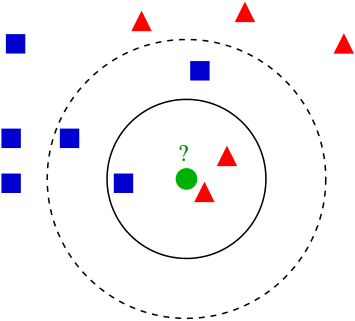
\includegraphics[width=0.7\linewidth]{img/knn_example}
	\caption{Esempio grafico dell'algoritmo KNN}
	\label{fig:knnexample}
\end{figure}


\subsubsection{Scelta del parametro k}
La scelta del parametro dipende, ovviamente, dal tipo dei dati che abbiamo e dalla quantita', anche se in generale piu' e' grande $k$ meno rumore viene generato da questo algoritmo. Un buon metodo per trovare il giusto valore e' l'uso di tecniche euristiche, come la \textit{cross validation}. Un altra fonte di rumore di cui bisogna stare attenti e' la presenza di \textit{features} insignificanti nella ricerca del vicino. Per porre rimedio possiamo, ad esempio, usare un algoritmo genetico per selezionare le \textit{features} piu' significative

\subsubsection{\textit{Curse of dimensionality}}
Un problema di cui soffrono vari modelli fra cui $knn$ e' la maledizione della dimensionalita' ovvero quando abbiamo dataset con elevata dimensionalita' come 50 attributi, modelli come $knn$ diventano molto imprecisi. Nel nostro classificatore la motivazione e' semplice: con tanti attributi la distanza tra punti incorrelati fra loro potrebbe diventare bassa soprattuto se presente del rumore nei dati oppure attributi insignificanti. Nel nostro problema non soffriamo della maledizione della dimensionalita' perche' abbiamo solo 3 attributi.

\subsection{Naive bayes}
Un altro tipo di apprendimento usato per classificare le \textit{label} e' Naive bayes: un algoritmo di classificazione e regressione basato sulla statistica. Prima di spiegare in cosa consiste occorre spiegare un paio di concetti:
\subsubsection{Teorema di bayes}
Il teorema di bayes ci fornisce una relazione fra probabilita' condizionate molto utile nel calcolo probabilistico ma anche per l'apprendimento automatico. L'equazione e' la seguente:
\begin{center}
	$P(B|A) = \dfrac{P(A|B)P(B)}{P(A)}$
\end{center}
\subsubsection{Rete bayesiana}
Una rete bayesiana e' un grafo diretto aciclico i cui nodi sono le variabili casuali del sistema mentre gli archi rappresentato la condizione di dipendenza fra nodi.
 Ad ogni nodo e' associata una tabella di distribuzione delle probabilita' la cui complessita' e' proporzionale al numero di archi entranti.\\ Per esempio se il nodo con variabile casuale Leggere ha un arco verso Istruito allora possiamo dire che Istruito e' condizionalmente dipendente da Leggere. Qui sotto potete vedere una raffigurazione grafica di una semplice rete bayesiana formata da nodi padre ed un figlio:
\begin{figure}[H]
	\centering
	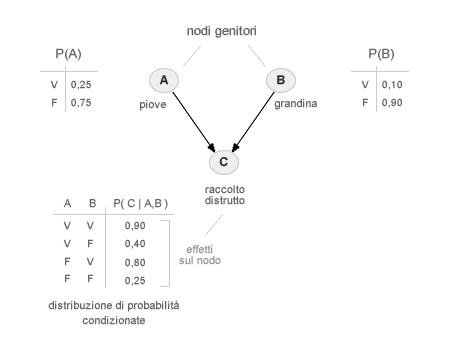
\includegraphics[width=0.7\linewidth]{img/rete-bayesiana-grafo.png}
	\caption{Esempio di rete bayesiana}
	\label{fig:rete-bayesiana-grafo}
\end{figure}
\medskip
\subsubsection{Naive Bayes}
Naive bayes e' una rete bayesiana in cui si assume l'indipendenza condizionale fra tutte le variabili casuali del sistema data la classe. Questa forte assunzione non mira a modellare esattamente la realta' ma nonostante cio' fornisce delle buone performance sulla predizione di una classe.

\begin{figure}[H]
	\centering
	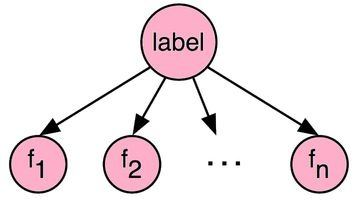
\includegraphics[width=0.4\linewidth]{img/naive_bayes_example}
	\caption{Esempio di rete bayesiana ingenua}
	\label{fig:naivebayesexample}
\end{figure}

\medskip


\subsubsection{Modelli generativi e discriminativi}
Una distinzione fra classificatori e' possibile farla nel modo in cui viene calcolata l'espressione $P(y_j|\textbf{x})$: nel caso di modelli discriminativi  (ad esempio \textit{knn} e alberi di decisione), l'obbiettivo e' discriminare, cioe' suddividere i dati originale per poter assegnare un'etichetta ai nuovi input mentre nei modelli generativi) l'obbiettivo e' di generare una distribuzione congiunta di probabilita' per $P(\textbf{x}, y_j)$ oppure da $P(\textbf{x}| y_j)$ e $P(y_j)$ per poter trovare l'etichetta piu' probabile. Fra questi ultimi ricade \textit{Naive Bayes}.

\subsubsection{Calcolo della probabilita' a priori}
  Per calcolare la probabilita' a priori esistono varie tecniche: l'equiprobabilita' $\left(\dfrac{1}{|\textbf{y}|}\right)$, rapporto fra esempi di classe $j$ e il totale degli esempi dall'insieme di addestramento, modelli ad eventi oppure un modello non parametrico dall'insieme di addestramento.
  
\subsubsection{Modelli ad eventi}  
   I modelli ad eventi sono distribuzioni di probabilita' che considerano gli attributi come probabilita' di eventi. Ci sono 3 modelli usati con $\textit{Naive Bayes}$ che sono:
\begin{itemize}
	\item Bernoulli: gli attributi sono di tipo \textit{booleano} e l'attributo $x_i \in \textbf{x}=(x_1,x_2,...,x_n)$ vale 1 se l'evento $i$ e' avvenuto, 0 altrimenti. Nel caso bernoulliano possiamo valutare $P(\textbf{x}|y_j)$ come
	\begin{center}
	 $P(\textbf{x}|y_j) = \prod_{j=1}^{n} P_{ij}^{x_i} (1-P_{ij})^{(1-x_i)}$
	\end{center}
	Dove $P_{ij}$ e' la probabilita' per $y_j$ che $x_i$ sia vero. Un esempio canonico e' quello della classificazione dei documenti, dove $x_i$ rappresenta la presenza del termine $w_j$ nei documenti di classe $y_j$ e di conseguenza $P_{ij}$ la probabilita' di trovarlo. Dobbiamo notar bene che Bernoulli a differenza della multinomiale valuta nella produttoria anche la probabilita' che l'evento $i$ non avvenga.
	

	\item Multinomiale: Nella multinomiale gli esempi rappresentano la frequenza con il quale gli eventi sono stati generati dalla multinomiale $(p_1...p_n)$ dove $p_i$ e' la probabilita' che $i$ occorra. Gli attributi $\textbf{x}=(x_1,x_2...x_n)$ contano quante volte l'evento $i$ e' avvenuto. La probabilita' condizionata  $P(\textbf{x}|y_j)$ e' stimata come
	\begin{center}
		$P(\textbf{x}|y_i) = \dfrac{(\sum_{i}x_i)!}{\prod_{i}x_i!}\prod_i p_{ki}^{x_i}$
	\end{center}
	\item Gaussiana: viene utilizzata con dati continui e si assume che siano distribuiti in base alla Gaussiana. Per ogni classe $y_j$, viene ricavata la media $\mu_j$ e la varianza $\sigma_{j}^{2}$. Supponiamo di aver raccolto un insieme di valori $v$ allora la probabilita' sara':
	\begin{center}
		$P(x =v | y_j) = \dfrac{1}{\sqrt{2 \pi \sigma_{j}^2}} e^{-\dfrac{(v - \mu_j)^2}{2 \sigma_{j}^2}}$
	\end{center}
	Un'altra possibile opzione per trattare valori continui e' la discretizzazione da cui possiamo utilizzare Bernoulli/Multinomiale anche se bisogna stare attenti a non perdere informazioni discriminanti.
\end{itemize}

\subsubsection{Un piccolo esempio basato su naive bayes}
Supponiamo di dover usare Naive Bayes per predire se giocare una partita di tennis o no in base alle condizioni meteorologiche. Dati gli esempi qui sotto a sinistra, possiamo ricavare la tabella di distribuzione delle probabilita' generale come qui di seguito:
\begin{figure}[H]
	\centering
	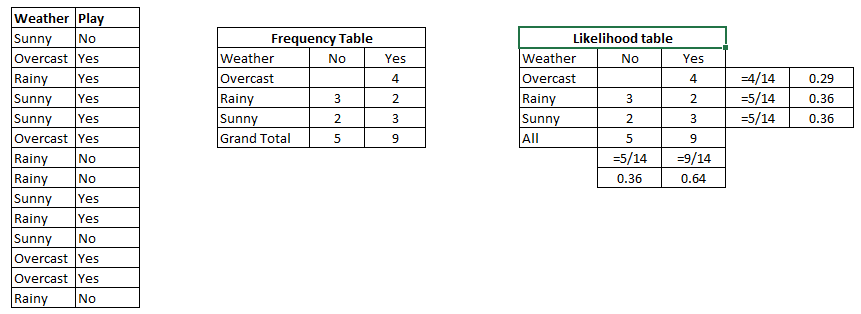
\includegraphics[width=1\linewidth]{img/Bayes_tennis_sample}
	\caption{Esempi di partite di tennis giocate in base alle condizioni meteorologiche e tabella di distribuzione delle probabilita'}
	\label{}
\end{figure}
\medskip
Ecco una rappresentazione grafica di \textit{Naive Bayes}:\\\\

\begin{figure}[H]
	\centering
	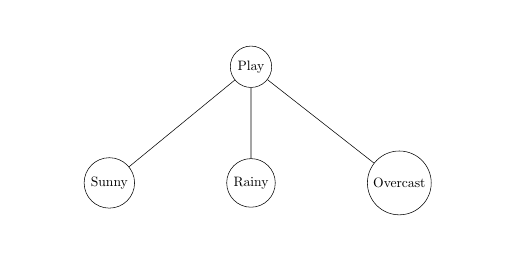
\includegraphics[width=0.7\linewidth]{img/graph_naive_bayes}
	\caption{Rappresentazione grafica di \textit{Naive bayes} nell'esempio del tennis}
	\label{fig:graphnaivebayes}
\end{figure}

%	\begin{tikzpicture} 
%		\node[draw, circle](0){Play}
%		child{ node(1)[draw, circle, left]{Sunny}}
%		child{	 	node(2)[draw, circle]{Rainy}}
%		child{	  node(3)[draw, circle, right]{Overcast} };
%	\end{tikzpicture}
\subsection{Alberi di decisione}
Da un punto di vista strutturale, l'albero di decisione e' un albero (inteso come struttura dati) dove i nodi interni sono gli attributi, i rami tutti i possibili valori assumibili dall'attributo (oppure un range nel caso continuo) e le foglie sono la predizione da scegliere.

\subsubsection{Classificazione dei nuovi elementi}
Quando dovremmo predire l'etichetta di un nuovo insieme di attributi $x$ bastera' semplicemente scorrere l'albero di decisione dalla radice fino ad una foglia, che sara' l'etichetta da assegnare.

\begin{figure}[H]
	\centering
	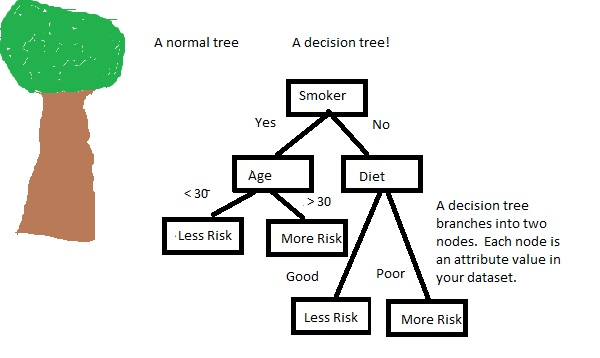
\includegraphics[width=0.7\linewidth]{img/dectree}
	\caption{Un albero e un albero di decisione a confronto. Nel secondo abbiamo come attributi \textit{Smoker, Age, Diet} e come etichetta \textit{Less Risk, More Risk} riferito alle malattie cardiache. }
	\label{fig:dectree}
\end{figure}


\subsubsection{Costruzione di un albero di decisione}
La costruzione dell'albero e' molto semplice: basta prendere gli attributi ed iniziare a suddividere a caso fino ad ottenere nodi con esempi di un solo tipo di etichetta.
In questo modo pero' otterremmo un albero  non molto utile in tutti i casi diversi dagli esempi. Quindi quale albero scegliere fra tutti quelli possibili? In questo caso ci aiuta un principio filosofico, il rasoio di Occam, che ci consiglia di scegliere quello piu' piccolo fra tutti. Per generare l'albero piu' piccolo dovremmo scegliere gli attributi piu' significativi per generare l'albero. Cosa intendiamo per significativo? Intendiamo l'attributo che genera figli con meno varieta' di classi presenti all'interno di essi, cioe' che discrimina meglio degli altri.\\ Un esempio: immaginiamo di avere 10 esempi con attributi A e B e come etichetta ${0,1}$. Ipotizziamo che suddividendo tramite l'attributo A avremmo due figli con esempi aventi meta' valore 0 e meta' 1 mentre se suddividiamo secondo B abbiamo nodi figli con esempi esclusivamente 1 oppure 0. In questo caso indubbiamente l'attributo piu' significativo e' B.\\Esistono vari criteri per misurare l'attributo piu' significato su cui suddividere il nodo che in termini tecnici vengono chiamate misure d'impurita'. Una misura e' l'indice di Gini il quale corrisponde alla seguente formula:
\begin{center}
	$\sum_{j} p(j|n)(1-p(j|n))$
\end{center}
dove $p(j|n)$ e' la percentuale di esempi con classe $j$ nel nodo $n$


\subsubsection{Un esempio di albero di decisione}
Riprendiamo l'esempio della partita di tennis, questa volta con qualche attributo in piu'. La tabella e' la seguente:
\begin{figure}[H]
	\centering
	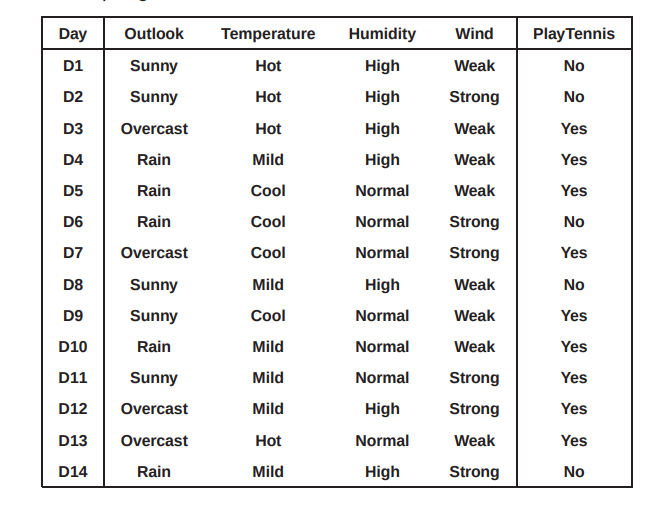
\includegraphics[width=0.7\linewidth]{img/decision-_tree_table_tennis}
	\caption{Tabella degli attributi meteorologici con valore associato un booleano che stabilisce se la partita e' stata giocata o no}
	\label{fig:decision-treetabletennis}
\end{figure}
da cui possiamo ricavare il seguente albero di decisione:
\begin{figure}[H]
	\centering
	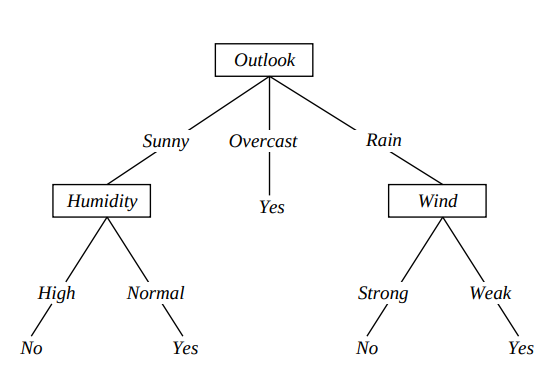
\includegraphics[width=0.7\linewidth]{img/decision_tree_tree_tennis}
	\caption{Albero di decisione ricavato dalla tabella precedente}
	\label{fig:decisiontreetreetennis}
\end{figure}

\section{Fase 3: Ricerca della posizione}
Dopo la costruzione del modello esso viene adoperato per predire la posizione corrente dell'utente che esegue l'applicazione. La ricerca consiste nel creare sul momento una \textit{fingerprint} e poi, tramite un algoritmo di classificazione, cercare di inferire la \textit{label}  su cui ci troviamo. Gli algoritmi utilizzati per analizzare il problema sono quelli descritti in precedenza quindi
\begin{enumerate}
	\item \textit{K Nearest Neightbour}
	\item Bayes ingenuo
	\item  Alberi di decisione
\end{enumerate}
\subsection{Ricerca di nuovi elementi nei classificatori}
Adesso vedremo come avviene la ricerca della posizione (quindi l'etichetta) nel Knn, naive bayes, alberi di decisione.
\subsubsection{\textit{K nearest neightbours}}
Preso un nuovo insieme di attributi $\overline{\textbf{x}}=\overline{x}_1\overline{x}_2\ldots\overline{x}_n$ saranno presi i primi k elementi che minimizzeranno la distanza euclidea tra $\overline{\textbf{x}}$ e tutti gli altri esempi gia' conosciuti precedentemente dal dataset d.
\begin{center}
	$\forall x \in d \,\,\,\min_k\,\,\, \sqrt{(\overline{\textbf{x}_1} - x_1)^2 + \ldots (\overline{\textbf{x}_n} - x_n)^2 }$
\end{center}

Una volta presi questi k elementi verra' trovata l'etichetta piu' frequente tra di essi e questa sara' l'etichetta di $\overline{\textbf{x}}$

\subsubsection{Naive bayes}

Preso un insieme di attributi $\textbf{x}$ con valori $x_1x_2x_3...x_n$ e tutti i valori possibili della variabile dipendente $\textbf{y}=y_1y_2y_3...y_m$ , per classificare l'insieme applicheremo il teorema di bayes con un'approssimazione molto usata nel campo scientifico chiamata MAP (Massima ipotesi a posteriori)
\begin{align*}
		etichetta &=y_j \, in \, \max_j\,P(y_j|X_1=x_1, X_2=x_2...X_N=x_n) \\
		&= \max_j \dfrac{P(X_1=x_1,X_2=x_2...X_N=x_n|y_j)P(y_j)}{P(X_1=x_1, X_2=x_2...X_N=x_n)}\\
		&= \max_j \dfrac{\prod_iP(x_i|y_j)P(y_j)}{P(X_1=x_1, X_2=x_2...X_N=x_n)}
\end{align*}

i cui valori della precedente equazione si possono ricavare dalla tabella di distribuzione delle probabilita'.

\subsubsection{Alberi di decisione}
Per ottenere la nuova etichetta di un insieme di attributi $\overline{\textbf{x}}$ e' sufficiente scorrere l'albero dalla radice fino ad uno dei nodi che sara' la nostra etichetta. Per scorrere l'albero e' sufficiente scegliere il ramo giusto in base al valore dell'attributo $\overline{\textbf{x}}$. Per fare un esempio pratico, in un certo nodo interno potremmo andare a sinitra se avessimo il valore di $x_3$ ed altrimenti a destra.